\chapter{Introduction}\label{ch:intro}

\def \path {other}
\def \imgpath {\path/images}

It has long been the goal of computer vision researchers to be able to develop
systems that can reliably recognize objects in a scene. Achieving this unlocks a huge
range of applications that can benefit society as a whole: fully
autonomous vehicles, automatic labelling of uploaded videos/images for
searching, interpretation and screening of security video feeds, and many more,
all far-reaching and extremely valuable. Many of these tasks are very tedious for humans
and would be done much better by machines if the missed-detection rate can be
kept low enough. The challenge does not lie in finding the
right application, but in the difficulty of training a computer to see.

Some of the difficulties associated with vision are the presence of nuisance
variables such as changes in lighting condition, changes in viewpoint, and
background clutter. These variables do not affect the scene but can drastically change the pixel
representation of it.
Humans, even at early stages of their lives, have little difficulty filtering
out these nuisance variables and are excellent at extracting the necessary information from a scene.
To design a robust system, it makes sense to take account of how our brains see
and understand scenes.

Unfortunately, biological vision is also a complex system. It has
more to it than simply collecting photons in the eye.
An excerpt from a recent Neurology paper \cite{raichle_two_2010} sums up the problem
well:

\begin{quotation}
It might surprise some to learn that visual information is significantly
degraded as it passes from the eye to the visual cortex. Thus, of the unlimited
information available from the environment, only about $10^{10}$ bits/sec are
deposited in the retina \ldots\ only $\sim 6\times 10^6$
bits/sec leave the retina and only $10^4$ make it to layer IV of V1
\cite{anderson_directed_2005,tor_norretranders_user_1998}. These data
clearly leave the impression that visual cortex receives an impoverished
representation of the world \ldots\ it should be noted that estimates of the
bandwidth of conscious awareness itself (i.e.,\ what we `see') are in the range
of 100 bits/sec or less\cite{anderson_directed_2005,
tor_norretranders_user_1998}.
\end{quotation}

Current video cameras somewhat act as a combination of the first and second
stage of this system, collecting photons in photosensitive sensors and then
converting this to a stream of images. Standard definition digital television
typically has
a bit rate between $3\x 10^6$ and $10^7$ bits/sec (slightly larger but comparable
to the $10^6$ bits/sec travelling through the optic nerve).

If we are to build effective vision systems, it makes sense to emulate this
compression of information between the optic nerve and the later stages of the visual
cortex.
% The question now stands before us --- what information is kept on entry to the V1 cortex?
Hubel and Wiesel revolutionized our understanding of the V1 cortex in their Nobel prize-winning work
(awarded in 1981 in Physiology/Medicine) by
studying cats \cite{hubel_receptive_1959, hubel_receptive_1962}, macaques and spider
monkeys \cite{hubel_receptive_1968}. They found that neurons in the V1 cortex fired
most strongly when edges of a particular (i.e.,\ neuron-dependent) orientation
were presented to the animal, so long as the edge was inside the receptive field of
this neuron.
Continuing on this work, Blakemore and Cooper \cite{blakemore_development_1970}
analysed the perception of kittens that had restricted visual information
presented to them.
In one of their experiments, the kittens were kept in darkness
and then exposed for a few hours a day to only horizontal or vertical lines.
After five months, they were taken into natural environments and their reactions
were monitored. The two groups of cats would only play with objects when
presented in an orientation that matched the orientation of their original
environment. This suggest that these early layers of perception are
\emph{learned}.
% A figure of the the frequency response of the photoreceptor cells in our eyes
% to different wavelengths of light.
% \begin{figure}
  % \begin{center}
      % 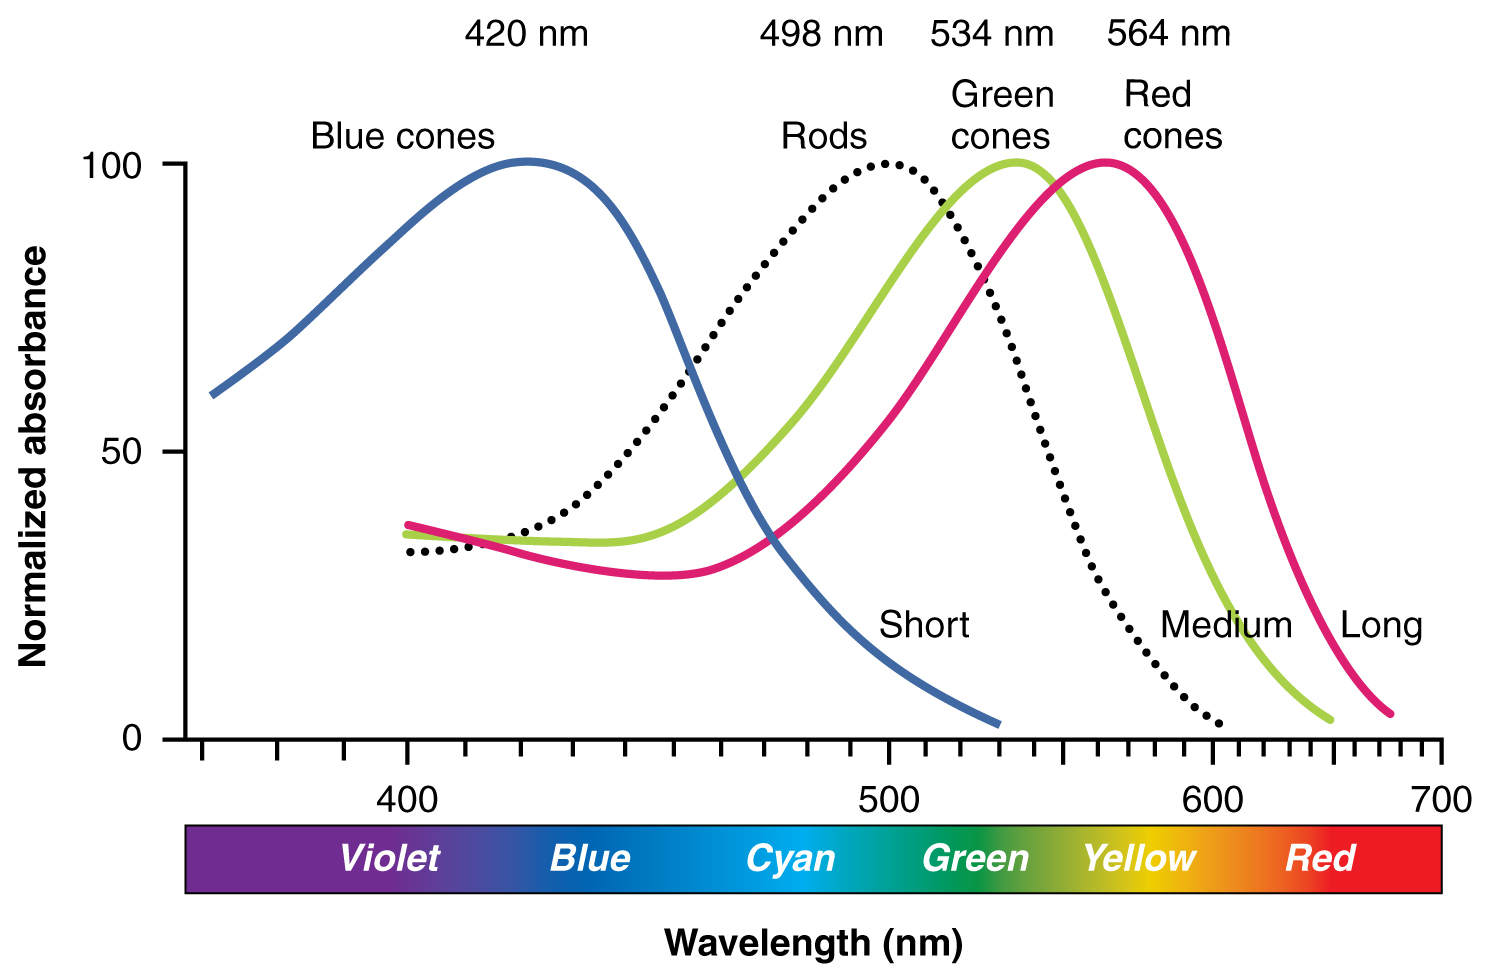
\includegraphics[width=10cm]{\imgpath/colour_sensitivity.jpg}
      % \mycaption{Frequency sensitivity of photoreceptors in they eye}
              % {Wavelength responsiveness of the different photoreceptors in the
               % eye. S, M, and L are short, medium, and long cones, compared to
               % R --- rods. Taken from~\cite{bowmaker_visual_1980}}
  % \end{center}
% \end{figure}

The current state of the art in image understanding systems are
Convolutional Neural Networks (CNNs). These are a learned model that
cascades many convolutional filters serially in layers, separated by
nonlinearities.
They are seemingly inspired by the visual cortex in the way that they are
hierarchically connected, progressively compressing the information into a
richer representation.

\autoref{fig:ch1:cnn_arch} shows an example CNN
architecture, the famous AlexNet \cite{krizhevsky_imagenet_2012}. Inputs are resized to a
manageable size, in this case, $224\x 224$ pixels. Multiple convolutional
filters of size $11\x 11$ are convolved over this input to give $96$ output
\emph{channels} (or \emph{activation maps}). In the figure, these are split onto two
graphics cards or GPUs for memory purposes. These are then passed through a
pointwise nonlinear function, or \emph{nonlinearity}.
The activations are pooled (a form of downsampling) and convolved with more
filters to give $256$ new channels at the second stage. This is repeated 3 more
times until the $13\x 13$ output with $256$ channels is unravelled and passed
through a fully connected neural network to classify the image as one of $1000$
possible classes.

CNNs have garnered lots of attention since 2012 when the previously mentioned AlexNet
nearly halved the top-5 classification error rate (from $26\%$ to $16\%$)
in the ImageNet Large Scale Visual Recognition Competition (ILSVRC)
\cite{russakovsky_imagenet_2014}\footnote{The previous state of
the art classifiers had been built by combining keypoint extractors like
SIFT\cite{lowe_distinctive_2004} and HOG\cite{dalal_histograms_2005} with
classifiers such as Support Vector Machines\cite{cortes_support-vector_1995} and
Fisher Vectors\cite{sanchez_image_2013}, for example \cite{sanchez_high-dimensional_2011}.}.
In the years since, the complexity of CNNs has grown significantly. AlexNet had
only 5 convolutional layers, whereas the 2015 ILSVRC winner ResNet \cite{he_deep_2016}
achieved 3.57\% top-5 error with 151 convolutional layers (and had some
experiments with 1000 layer networks).

\begin{figure}
  \centering
    % \includegraphics[width=\textwidth]{\imgpath/dtcwt_gain}
    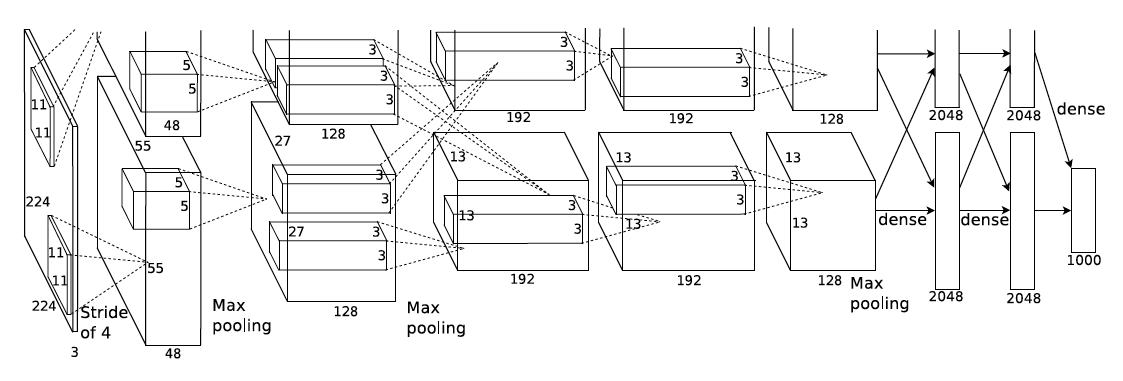
\includegraphics[width=\textwidth]{\imgpath/alexnet.png}
    \mycaption{Convolutional Architecture example}{The previous layer's activations are
    combined with a learned convolutional filter.
    Note that while the activation maps are 3-D arrays, the convolution is only
    a 2-D operation. This means the filters have the same number of channels as
    the input and produce only one output channel. Multiple channels are made by
    convolving with multiple filters. Not shown here are the nonlinearities that
    happen in between convolution operations. Image taken from \cite{krizhevsky_imagenet_2012}.}
    \label{fig:ch1:cnn_arch}
  \end{figure}

\section{Motivation}\label{sec:ch1:motivation}
\begin{figure}
  \centering
  \subfloat[conv1 filters]{
  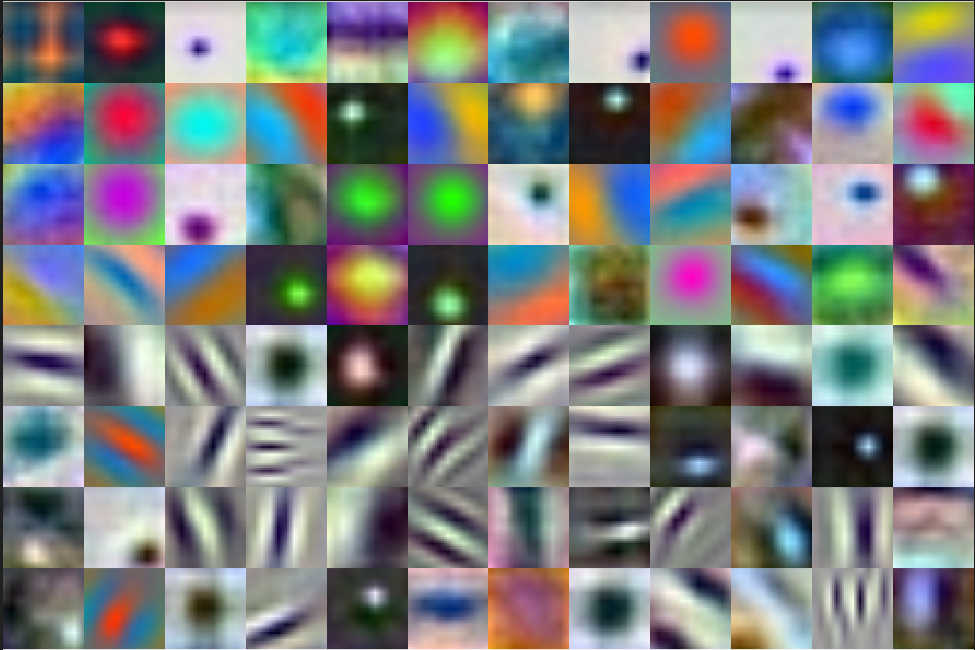
\includegraphics[width=0.6\textwidth]{\imgpath/alexfilters.png}
  \label{fig:ch1:alex_filt}
  }\\
  \subfloat[conv1 activations]{
  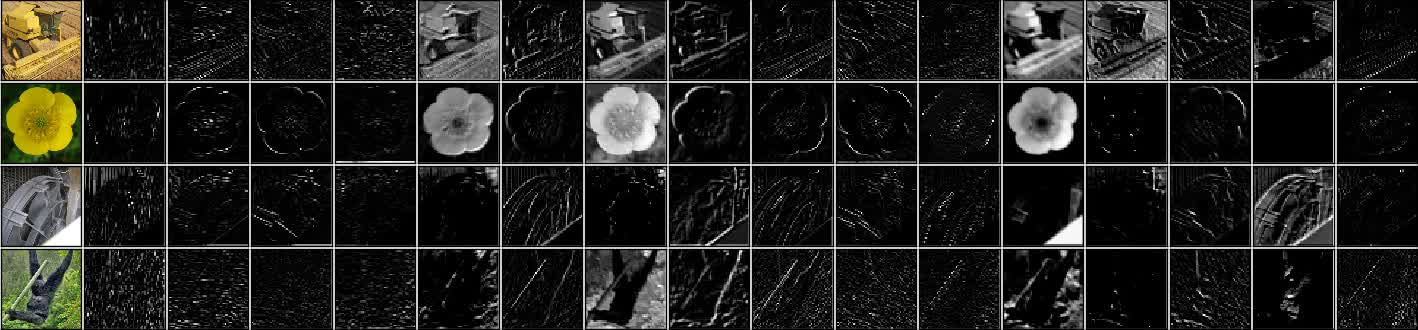
\includegraphics[width=\textwidth]{\imgpath/out1.jpg}
  \label{fig:ch1:alex_conv1}
  }\\
  \subfloat[conv2 activations]{
  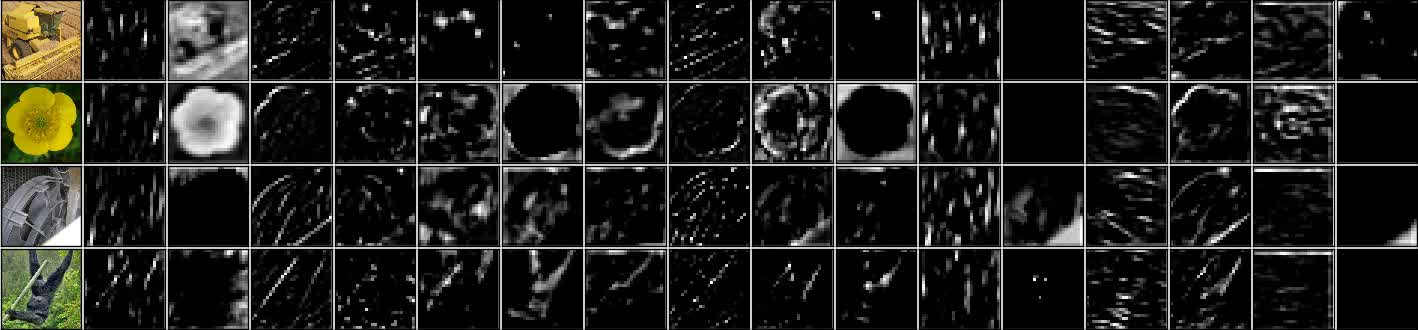
\includegraphics[width=\textwidth]{\imgpath/out2.jpg}
  \label{fig:ch1:alex_conv2}
  }\\
  \subfloat[conv3 activations]{
  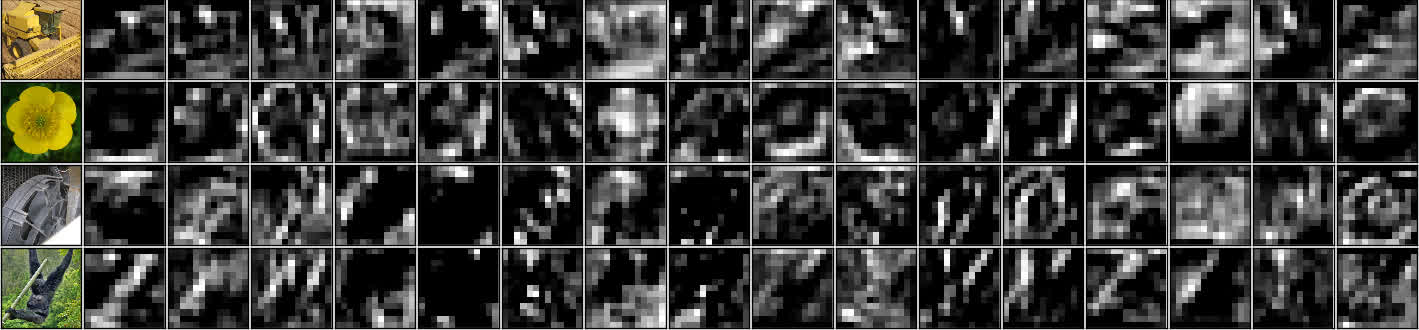
\includegraphics[width=\textwidth]{\imgpath/out3.jpg}
  \label{fig:ch1:alex_conv3}
  }
  \mycaption{Example first layer filters and the first three
  layer's outputs}{\subref{fig:ch1:alex_filt} The $11\x 11$ filters for the
  first stage of AlexNet. Of the 96 filters, 48 were learned on one GPU and
  another 48 on another GPU. Interestingly, one GPU has learned mostly
  lowpass/colour filters and the other has learned oriented bandpass
  filters. \subref{fig:ch1:alex_conv1} - \subref{fig:ch1:alex_conv3} Randomly
  chosen activations from the output of the first, second and third convolutional
  layers of AlexNet (see \autoref{fig:ch1:cnn_arch}) with negative values set to 0.
  Filters and activation images taken from supplementary material of
    \cite{krizhevsky_imagenet_2012}.}
  \label{fig:ch1:alexnet_filters}
\end{figure}

Despite their success, CNNs are often criticized for being \emph{black-box}
methods. You can view the first layer of filters
quite easily (see \autoref{fig:ch1:alex_filt}) as they exist in RGB
space, but beyond that things get trickier as the filters have a third, \emph{channel}
dimension, typically much larger than the two spatial dimensions. Additionally,
it is not clear what the input channels themselves correspond to. For illustration
purposes, we have also shown some example activations from the first three
convolutional layers for AlexNet in
\autoref{fig:ch1:alexnet_filters}\subref{fig:ch1:alex_conv1}-\subref{fig:ch1:alex_conv3}\footnote{These activations are
taken after a specific nonlinearity that sets negative values to 0, hence the
large black regions.}. For the conv1 activations in
\autoref{fig:ch1:alex_conv1}, we can accurately guess that some of the first layer
channels are responding to edges or colour information, but as we go deeper to
conv2 and conv3, it becomes less and less clear what each activation is
responding to.

This has started to become a problem, and while we are happy to trust modern
CNNs for isolated tasks, we are less likely to be comfortable with them driving
cars through crowded cities, or making executive decisions that affect people
directly. In a commonly used contrived example, it is not hard to imagine a deep
network that could be used to assess whether giving a bank loan to an applicant
is a safe investment. Trusting a black box solution is deeply unsatisfactory in
this situation. Not only from the customer's perspective, who, if declined, has
the right to know why \cite{goodman_european_2016}, but
also from the bank's --- before lending large sums of money, most banks
would like to know why the network has given the all clear. `It has worked well
before' is a poor rule to live by.

Aside from their lack of interpretability, it often takes a long time and a lot of
effort to train state-of-the-art CNNs. Typical networks that have won ILSVRC
since 2012 have had roughly 100 million parameters and take up to a week to train. This
is optimistic and assumes that you already know the necessary optimization or
architecture hyperparameters, which you often have to find out by trial and error.
In a conversation the author had with Yann LeCun, the attributed father of
CNNs, at a Computer Vision Summer School (ICVSS 2016), LeCun highlighted this problem
himself:
\begin{quote}
  There are certain recipes (for building CNNs) that work and certain recipes
  that don't, and we don't know why.
\end{quote}

Considering the recent success of CNNs, it is becoming more and more
important to understand \emph{how} and \emph{what} a network learns, so we can
interrogate what in the input has contributed to it making its classification or regression choice.
Without this information, the use of these incredibly powerful tools could be
restricted to research and proprietary applications.

\section{Approach}
The structure of convolutional layers is fairly crude in terms of signal
processing - arbitrary taps of an FIR filter are learned typically via
stochastic gradient descent from random starting states to minimize either a
mean-squared error or cross-entropy loss.

This leads us to ask a motivating question:
%
\begin{quote}
  Is it possible to learn convolutional filters as combinations of basis
  functions rather than individual filter taps?
\end{quote}

In achieving this, it is important to find ways to have an adequate
richness of filtering while reducing the number of parameters needed to specify resulting
filters. We want to contract the space of learning to a subspace or manifold that
is more useful. In much the same way, the convolutional layer in a CNN is a restricted
version of a fully connected layer in a multi-layer perceptron, yet adding this
restriction allowed us to train more powerful networks.

\begin{quote}
The intuition that we explore in this thesis is that \emph{complex wavelets} are
good basis functions for filtering in CNNs.
\end{quote}

\subsection{Why Complex Wavelets?}
Most modern approaches to CNNs are framed entirely in the spatial domain; our
choice of complex wavelets as the basis function to explore comes from the
deeper intuition that it may be helpful to rethink about CNNs in the
\emph{frequency domain}.  Historically, the frequency domain has been an
excellent space for solving many signal processing problems such as noise
removal, filter design, edge detection and data compression. We believe it may prove to
have advantages for CNNs too (beyond just an efficient space to do convolution
in).

The Fourier transform, which uses complex sinusoids as
its basis function, is perhaps the most ubiquitous tool to use for frequency
domain analysis. The problem with these complex sinusoids is that they have
\emph{infinite} support. This means that small changes in one part of an image
affect every Fourier coefficient. Additionally, they are not stable to small
deformations, as small changes can produce unbounded changes in the representation
\cite{mallat_group_2012}.

The common remedy to this problem is to use the localized, and more
stable, short-time Fourier transform (STFT). The STFT (or the Gabor transform)
is a natural extension of the Fourier transform, windowing the complex sinusoids
with a Gaussian (or similar) function. The STFT has the undesirable property that all
frequencies are sampled with the same resolution. A close relative of the STFT is the
continuous wavelet transform (CWT). The shorter duration of the wavelet basis
functions as the frequency increases means that their time resolving power
improves with centre-frequency.
Another commonly used
wavelet transform is the discrete wavelet transform (or the DWT) often favoured over
the CWT because of its speed of computation. It can use many
different finite support basis functions, all with different frequency
localization properties, but it is usually limited to using real filters. As such, it
suffers from many problems such as shift-dependence and lack of directionality in
two dimensions (2-D). These problems can be remedied by using the slower CWT with complex basis
functions, but we choose instead to use the dual-tree complex wavelet transform,
or $\DTCWT$ \cite{selesnick_dual-tree_2005} with q-shift filters \cite{kingsbury_complex_2001}.

The $\DTCWT$ allows for complex basis functions that have shift-invariance and
directionality, while being fast to implement like the DWT (in 2-D it can be thought of as the
application of 4 DWTs in parallel). It is also more easily invertible than the
CWT, forming a tight frame \cite{kovacevic_introduction_2008}, which we believe
may prove to be a very important property for visualizing what a
CNN is responding to.

We revisit the properties of the Fourier transform, STFT, CWT, DWT and $\DTCWT$
and expand on the properties behind our choice of basis functions
in the literature review \autoref{sec:ch2:fourier}.

On top of the intuition that the wavelet domain is a good space in which to frame CNNs,
there are some experimental motivating factors too. Firstly, the wavelet
transform has had much success in image and video compression, particularly for
JPEG2000 \cite{taubman_jpeg2000_2013}. Good compression performance implies an ability of
the basis functions to represent the input data sparsely (as seems to happen in
the brain). Secondly, the filters from the first layer of AlexNet
(\autoref{fig:ch1:alexnet_filters}) look like oriented wavelets. Given that
there was no prior placed on the filters to make them have this similarity to
wavelets, this result is noteworthy. And finally, the aforementioned work of
Hubel and Wiesel suggests that the early layers of the visual system act like a
Gabor transform.

These experimental observations imply that complex wavelets would do well in
replacing the first layer of a CNN, but we would aslo like to find out if they can be used
at deeper layers. Their well-understood and well-defined behaviour would help us
to answer the above \emph{how} and \emph{why} questions. Additionally, they
allow us to enforce a certain amount of smoothness and near orthogonality;
smoothness seems to be important to avoid sensitivity to adversarial or spoofing
attacks \cite{szegedy_intriguing_2014} and near orthogonality allows you to
cover a large space with fewer coefficients.

But first, we must find out \emph{if} it is possible to get the same or nearly the same
performance by using wavelets as the building blocks for CNNs, and this is the
core goal of this thesis.

\section{Method}
\subsection{ScatterNets}
To explore the uses of complex wavelets in CNNs, we begin by looking at one of the most
popular current uses of wavelets in image recognition tasks, the
Scattering Transform.

The Scattering Transform, or the \emph{ScatterNet}, was introduced in \cite{mallat_group_2012,
bruna_invariant_2013} at the same time as AlexNet. It is a non-black-box
network that can be thought of as a restricted complex-valued CNN
\cite{bruna_mathematical_2015}. Unlike a CNN, it has predefined
convolutional kernels, set to complex wavelet (and scaling) functions and uses
the complex magnitude as its nonlinearity. Due to
its well-defined structure, it can be analyzed and bounds on its stability to
shifts, noise and deformations are found in \cite{mallat_group_2012}.
%
% This is a promising start to addressing the problems of CNNs as using
% predefined, general filters helps us answer \emph{how} a CNN is
% learning, although the \emph{what} is still somewhat unclear.

For a simple task like identifying small handwritten digits,
the variabilities in the data are simple and small and the ScatterNet can easily
reduce the problem into a space which a Gaussian Support Vector Machine (or SVM
\cite{cortes_support-vector_1995}) can easily solve
\cite{bruna_invariant_2013}. For a more complex task like identifying real-world
objects, the ScatterNet can somewhat reduce the variabilities and get good
results with an SVM, but there is a significant performance gap between this and
what a CNN can achieve. For example, in \cite{oyallon_deep_2015} a second-order
ScatterNet can achieve $82.3\%$ top-1 classification accuracy on CIFAR-10, a
commonly used dataset, whereas modern CNNs such as \cite{he_deep_2016} can
achieve $93.4\%$.

\subsection{Learnable ScatterNets}
To start to address the performance gap between ScatterNet front ends and CNNs
we first investigate the properties of current ScatterNets. Inspired by the
visualization work of \citeauthor{zeiler_visualizing_2014}
\cite{zeiler_visualizing_2014} we build a DeScatterNet. The DeScatterNet
leverages the perfect reconstruction properties of the $\DTCWT$ and allows us to
investigate what in the input image the ScatterNet is responding to.

The DeScatterNet shows that the ScatterNet may be limiting itself by not
combining the filtering of different wavelet orientations (it does not mix the
channels as a CNN does). Inspired by the work of \cite{qiu_dcfnet:_2018}, we
propose the learnable ScatterNet, which includes this mixing while keeping the
desirable properties of the ScatterNet.

The learnable ScatterNet can be thought of as using the scattering outputs as
the \emph{basis functions}\footnote{Although they are not true basis functions
as they are the combination of a complex wavelet with a modulus nonlinearity,
and are thus data-dependent.} for our convolutional layers. We show that this
improves greatly on the ScatterNet design, and under certain constraints can
improve on the performance of CNNs too.

\subsection{Wavelet Domain Filtering}
We find that the complex modulus of the ScatterNet design to be useful for some
operations in a CNN, but it has a demodulating effect on the frequency energy
(all the outputs have significantly more energy in lower frequencies). This
limits repeated application of it as the demodulating effect compounds.

We develop a system that does not use the complex modulus; instead, it
learns \emph{complex} gains in the wavelet domain.
Rather than mixing subbands together, we keep them independent and only learn to
mix across the channel dimension. This is important, as it allows us to then use the inverse
$\DTCWT$ to return to the pixel domain. The shift-invariant properties of the $\DTCWT$ mean the
reconstructed outputs are (mostly) free from aliasing effects, despite much of
the processing being carried out at significantly reduced sample rates in the
wavelet domain.

We show that our layer can be used alongside regular convolutional
layers. I.e., it becomes possible to `step' into the wavelet domain to do
wavelet filtering for one layer, before `stepping' back into the pixel domain to
do pixel filtering for the next layer.

\section{Thesis Layout and Contributions to Knowledge}
This thesis has one literature review chapter and four novel-work chapters:
\begin{itemize}
\item
  \hyperref[ch:litreview]{Chapter~\ref*{ch:litreview}}
  explores some of the background necessary for starting
  to develop image understanding models. In particular, it covers the
  inspiration for CNNs and the workings of CNNs themselves, as well as covering
  the basics of wavelets and ScatterNets.
\item
  \Autoref{Chapter}{ch:dtcwt_scat} proposes a change to the core of the ScatterNet. In
  addition to performance issues with ScatterNets, they are slow and both
  memory-intensive and compute-intensive to calculate. This in itself is enough of an
  issue to make it unlikely that they would be used as part of deep networks. To
  overcome this, we change the computation to use the $\DTCWT$
  \cite{selesnick_dual-tree_2005} instead of Morlet wavelets, achieving a 20 to
  30 times speed-up while achieving a small improvement in classification performance.
\item
  \Autoref{Chapter}{ch:visualizing} describes our \emph{DeScatterNet}, a tool used to
  interrogate the structure of ScatterNets. We also perform tests to determine
  the usefulness of the different scattered outputs finding that many of them
  are not useful for image classification.
\item
  \Autoref{Chapter}{ch:invariant} describes the \emph{Learnable ScatterNet} we have developed to
  address some of the issues found from the interrogation in
  \autoref{ch:visualizing}. We find that a learnable ScatterNet layer performs
  better than a regular ScatterNet, and can improve on the performance of a CNN
  if used instead of pooling layers. We also find that scattering works well not
  just on RGB images, but can also be useful when used after one layer of
  learning.
\item
  In \autoref{ch:freqlearn}, we step away from ScatterNets and present the
  \emph{Wavelet Gain Layer}. The gain layer uses
  the wavelet space as a latent space to learn representations. We find possible
  nonlinearities and describe how to learn in both the pixel and wavelet domain.
  This work showed that there may well be benefits to learning in the wavelet
  domain for earlier layers of CNNs, but we have not yet found advantages to
  using the wavelet gain layer for deeper layers.
\end{itemize}

\subsection{Contributions and Publications}
The key contributions of this thesis are:

\begin{itemize}
  \item Software for wavelets and $\DTCWT$ based ScatterNet (described in \autoref{ch:dtcwt_scat})
    and publicly available at \cite{cotter_pytorch_2018}.
  \item ScatterNet analysis and visualizations (described in
    \autoref{ch:visualizing}). This chapter expands on the paper we presented at MLSP2017
    \cite{cotter_visualizing_2017}.
  \item Invariant Layer/Learnable ScatterNet (described in \autoref{ch:invariant})). This chapter expands
    on the paper accepted at ICIP2019 \cite{cotter_learnable_2019}. Software
    available at \cite{cotter_learnable_2019-1}.
  \item Learning convolutions in the wavelet domain (described in
    \autoref{ch:freqlearn}). We have published preliminary results on this work
    to arXiv \cite{cotter_deep_2018} but have expanded on this paper in the
    chapter. Software available at \cite{cotter_dtcwt_2018}.
\end{itemize}

\subsection{Related Research}
Readers may also be interested in the theses \cite{singh_scatternet_2018} and
\cite{oyallon_analyzing_2017}.

In \cite{singh_scatternet_2018}
\citeauthor{singh_scatternet_2018} looks at using the ScatterNet as a fixed
front end and combining it with well-known machine learning methods such as
SVMs, Autoencoders and Restricted Boltzmann Machines. By combining frameworks in
a defined way he creates unsupervised feature extractors which can then be used
with simple classifiers. Some relevant papers that makeup this thesis are \cite{singh_multi-resolution_2016,
singh_scatternet_2017, singh_generative_2018}. In
\cite{singh_multi-resolution_2016} Singh shows
that the $\DTCWT$-ScatterNet outperforms a Morlet-ScatterNet when used as a front end for
an SVM, which is similar to the work we do in \autoref{ch:dtcwt_scat} where we
show the $\DTCWT$-ScatterNet outperforms a Morlet-ScatterNet when used as a
front end for CNNs. He then expands on this work by testing other backends in
\cite{singh_scatternet_2017, singh_generative_2018}.

In \cite{oyallon_analyzing_2017}
\citeauthor{oyallon_analyzing_2017} looks at ScatterNets as front ends to
deeper learning systems, such as CNNs. Some relevant papers that makeup Oyallon's thesis are
\cite{oyallon_deep_2015, oyallon_scaling_2017, oyallon_hybrid_2017}. \cite{oyallon_scaling_2017, oyallon_hybrid_2017}
are particularly relevant as he uses a ScatterNet as a feature extractor for a
CNN. We do similar research in \autoref{ch:invariant}, but allow for
learned weights in the ScatterNet in our design.
